\section{FLASH-RT}

    %%%%%%%%%%%%%%%%%%%%%%%%%%%%%%%%%%%%%%%%
    %%  Slide 1: <>  %%
    %%%%%%%%%%%%%%%%%%%%%%%%%%%%%%%%%%%%%%%%
    \begin{frame}
        \frametitle{FLASH radiotherapy}
        \begin{itemize}
            \item Radiotherapy takes advantage of the damage caused by the ionization of energy loss by particles
            \item FLASH-RT consists in delivering a high level of dose in a small fraction of time: this seems reducing the toxiticy of the radiation on healty tissues
        \end{itemize}
        \medskip
        \begin{columns}
            \column{0.5\textwidth}  
                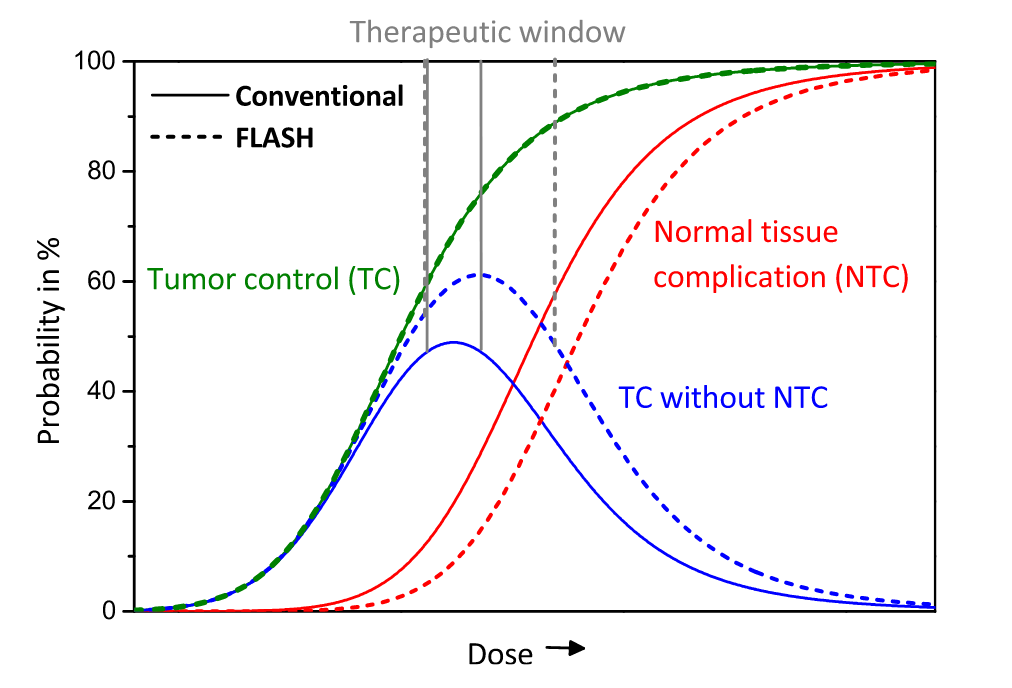
\includegraphics[width=1.25\linewidth]{figures/pixel_detectors_usage/curve_flash.png}
        \column{0.5\textwidth}
            
            \begin{itemize}
                \item FLASH-RT is still \textbf{under test}!
                \begin{itemize}
                    \item medical aspect%: in vitro and with animals; only one patient has been treated
                    \item  bio-physics aspect%: dependence of the FLASH effect on the treatment conditions 
                    \item  strumental aspect%: need for new detectors
                \end{itemize}
            \end{itemize}
        \end{columns}
    \end{frame} 


    %%%%%%%%%%%%%%%%%%%%%%%%%%%%%%%%%%%%%%%%
    %%  Slide 1: <>  %%
    %%%%%%%%%%%%%%%%%%%%%%%%%%%%%%%%%%%%%%%%
    \begin{frame}
        \frametitle{Electron FLASH radiotherapy}
        \centering
        \bigskip
        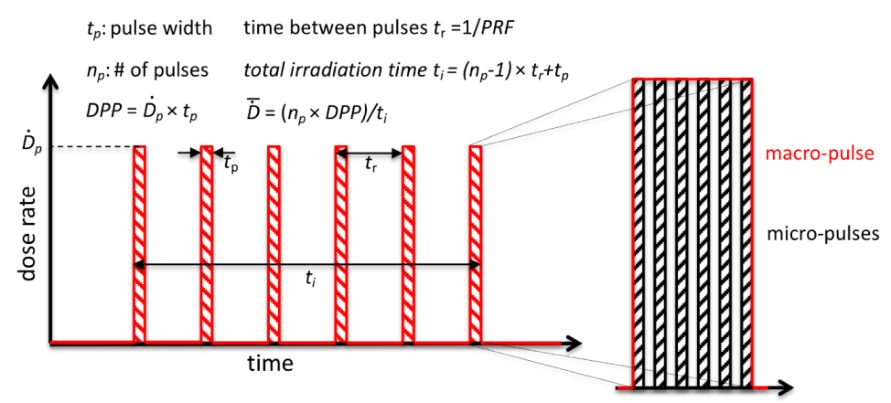
\includegraphics[width=.9\linewidth]{figures/test_beam/beam_structure.pdf}
        \begin{columns}
            \column{0.8\textwidth}
                \begin{table}
                    \footnotesize
                    \begin{center}
                    \begin{tabular}{|c | c |c |}
                    \hline
                    & CONV-RT & FLASH-RT \\
                    \hline
                    \hline
                    Dose rate & \SI{0.03}{Gy/s} & \SI{40}{Gy/s}\\
                    Intra pulse dose rate & \SI{100}{Gy/s}&\SI{10 6}{Gy/s}\\
                    Treatment duration & $\sim$minutes & $\lessapprox$\SI{500}{ms} \\
                    Dose Per Pulse & \SI{0.3}{Gy} & 1-10 Gy\\
                    Pulse width & \SI{3}{\us} & $\sim$\SI{2}{\us} \\
                    \hline
                    \end{tabular}
                    \end{center}
                \end{table} 
                
            \column{0.3\textwidth}
                Assuming \textbf{water} as the dosimetric reference material 
                %\begin{equation*}
                %    N_A[/\si{\cm\squared}] = \frac{DPP[Gy]}{10^{10} S[\si{MeV \cm \squared /g}]}
                %\end{equation*}
        \end{columns}
    \end{frame}     


    %%%%%%%%%%%%%%%%%%%%%%%%%%%%%%%%%%%%%%%%
    %%  Slide 1: <dosimeters>  %%
    %%%%%%%%%%%%%%%%%%%%%%%%%%%%%%%%%%%%%%%%
    \begin{frame}
        \frametitle{FLASH-RT: need for detectors}
        All online detector types show saturation problems at such high intensity
        \medskip
        \begin{columns}
            \column{0.4\textwidth} 
            Different types of detector with different charateristics are required: 
                \begin{itemize}
                    \item \textbf{dosimeters} 
                    \item \textbf{beam monitors} 
                    \item detectors for diagnostic 
                \end{itemize}
            \column{0.6\textwidth}  
                \hspace*{-0.6cm}
                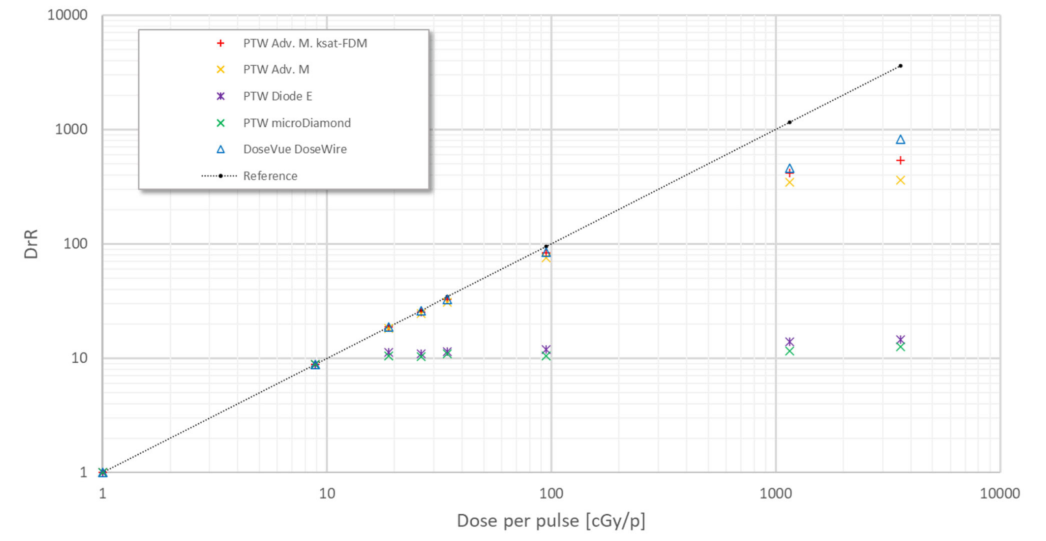
\includegraphics[width=1.15\linewidth]{figures/pixel_detectors_usage/saturation_dosimeters.pdf}
                %COSA SONO I COLORI
                Rif.articolo\\\bigskip
                \hspace*{-3.cm}$N_A$ = 0.2-1.2 10$^9$/cm$^2$ @ Dose Per Pulse = 0.07-0.4 Gy
        \end{columns}
    \end{frame}     



    %%%%%%%%%%%%%%%%%%%%%%%%%%%%%%%%%%%%%%%%
    %%  Slide 1: <dosimeters>  %%
    %%%%%%%%%%%%%%%%%%%%%%%%%%%%%%%%%%%%%%%%
    \begin{frame}
        \frametitle{Possible applications of MAPS}
        \begin{enumerate}
            \item \textbf{Dosimeters}: very difficult because of saturation effect. \\
            Need to: 
            \begin{itemize}
                \item divide the charge of one pulse in microbuckets
                \item reduce the FE charge sensitivity by large factor 
                \item use a fast FE and a fast readout
            \end{itemize}
            \bigskip
            \item \textbf{Beam position monitors}: very thin detectors ($\sim$\SI{50}{\um}) with low disturbance 
                \begin{itemize}
                    \item \textbf{Very High Energy Electrons FLASH-RT} that uses pencil beams, in this case the pixels are saturated but it does not matter
                \end{itemize}
        \end{enumerate}
    \end{frame}     


    %%%%%%%%%%%%%%%%%%%%%%%%%%%%%%%%%%%%
    %% Slide 2: <> %%
    %%%%%%%%%%%%%%%%%%%%%%%%%%%%%%%%%%%%
    \begin{frame}
        \frametitle{Test on the beam: experimental set up}
        \smallskip
        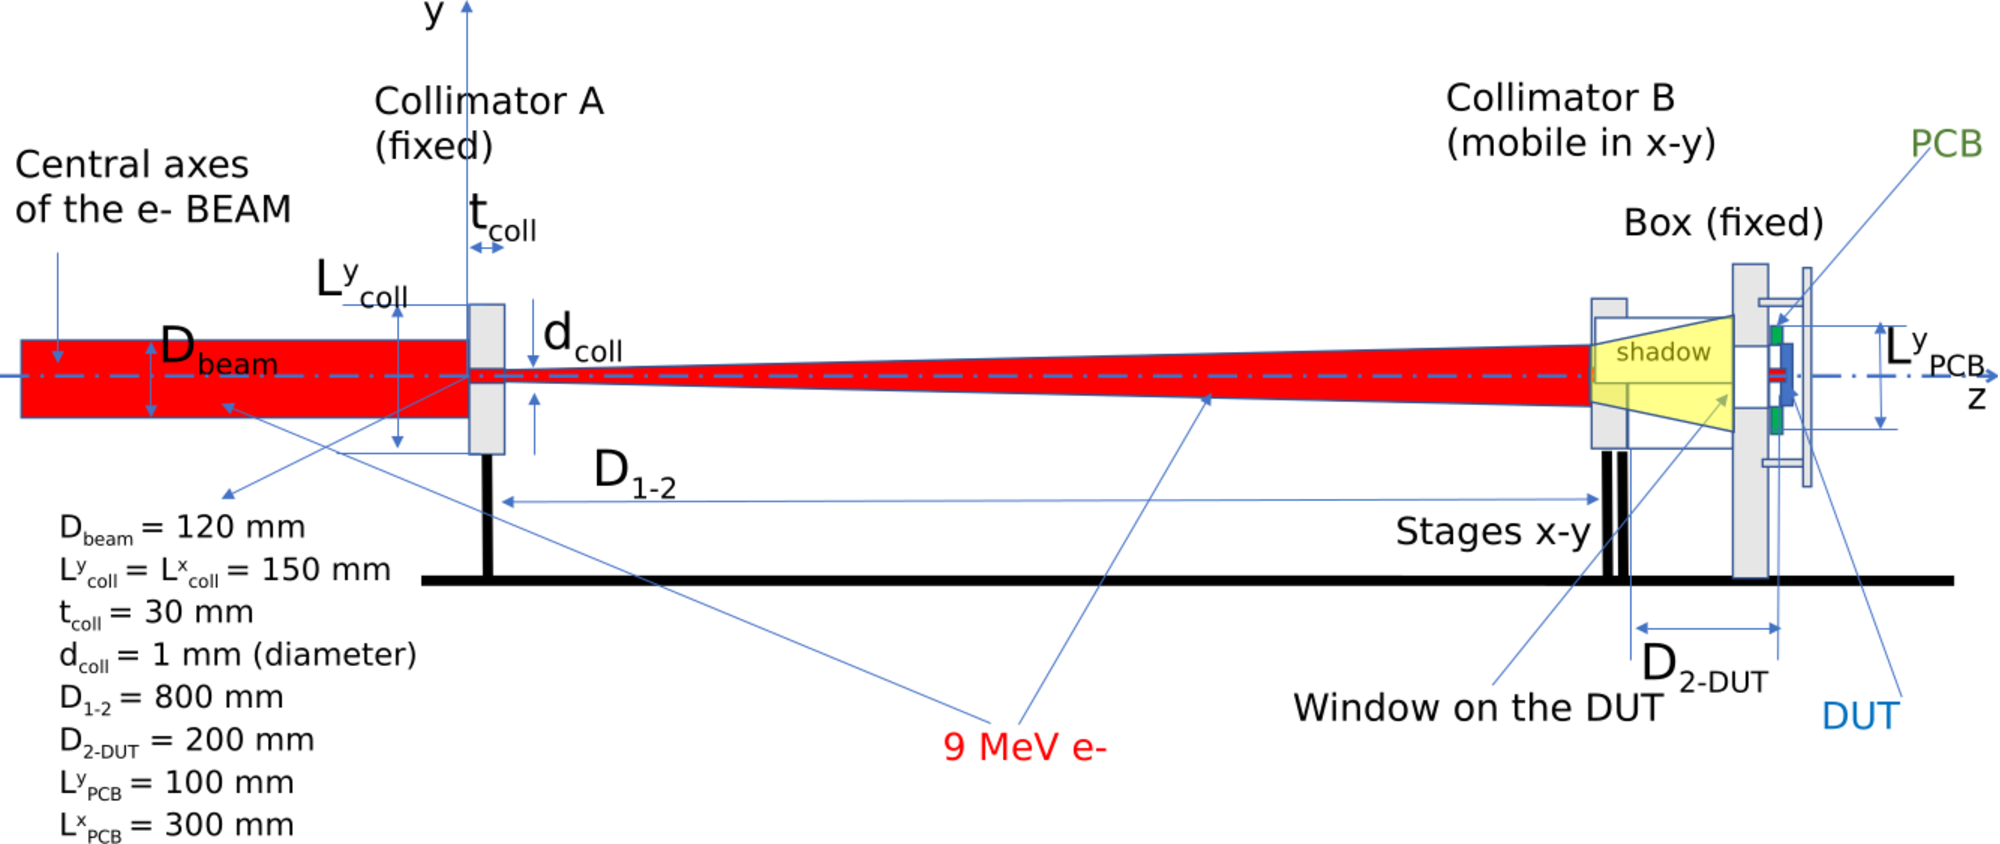
\includegraphics[width=.95\linewidth]{figures/test_beam/Flash-beam-scheme.pdf}\\
        \smallskip
        \begin{enumerate}
            \item Collimator A: to reduce fluence on the DUT of \textbf{4 10$^{-4}$}
            \item Collimator B: to illuminate only a small portion of DUT to see the beam border
        \end{enumerate}
        %$N_A$ = 2.9 10$^9$/cm, F = 7.25$\times$10$^{9}$\si{MHz/cm\squared} @  DPP=\SI{1}{Gy}, t$_p$=\SI{4}{\us}
        
    \end{frame}    


    %%%%%%%%%%%%%%%%%%%%%%%%%%%%%%%%%%%%
    %% Slide 2: <> %%
    %%%%%%%%%%%%%%%%%%%%%%%%%%%%%%%%%%%%
    \begin{frame}
        \frametitle{Test on the beam: experimental set up}
        \centering
        \includegraphics[width=.7\linewidth]{figures/test_beam/testbeam_photos.pdf}  
    \end{frame}    

    %%%%%%%%%%%%%%%%%%%%%%%%%%%%%%%%%%%%
    %% Slide 2: <> %%
    %%%%%%%%%%%%%%%%%%%%%%%%%%%%%%%%%%%%
    \begin{frame}
        \frametitle{Test on the beam: preliminary results}
        \begin{columns}
            \column{0.5\textwidth} 
                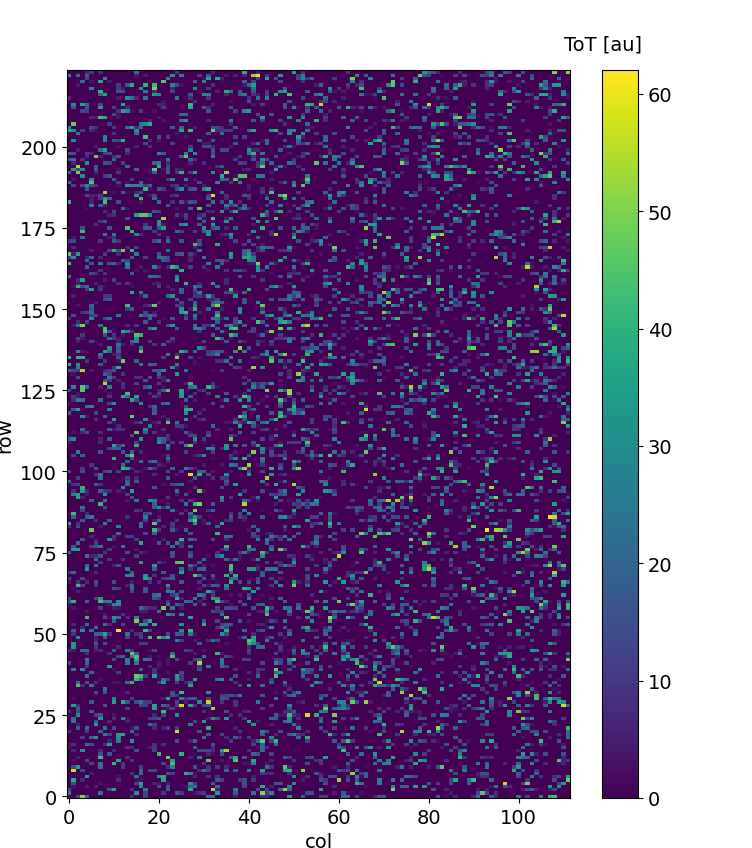
\includegraphics[width=1.1\linewidth]{figures/test_beam/tot_mapq1_15-57.png}  
            \column{0.5\textwidth} 
                \begin{itemize}
                    \item Under-extimation of the Bremsstrahlung production of electrons which stop in the collimators 
                    \item High background in data
                    \item Need for a simulation to better understand the data
                \end{itemize}
            \end{columns}
        \end{frame}  


    %%%%%%%%%%%%%%%%%%%%%%%%%%%%%%%%%%%%
    %% Slide 2: <> %%
    %%%%%%%%%%%%%%%%%%%%%%%%%%%%%%%%%%%%
    \begin{frame}
        \frametitle{Test on the beam: preliminary results}
        \begin{columns}
            \column{0.5\textwidth} 
                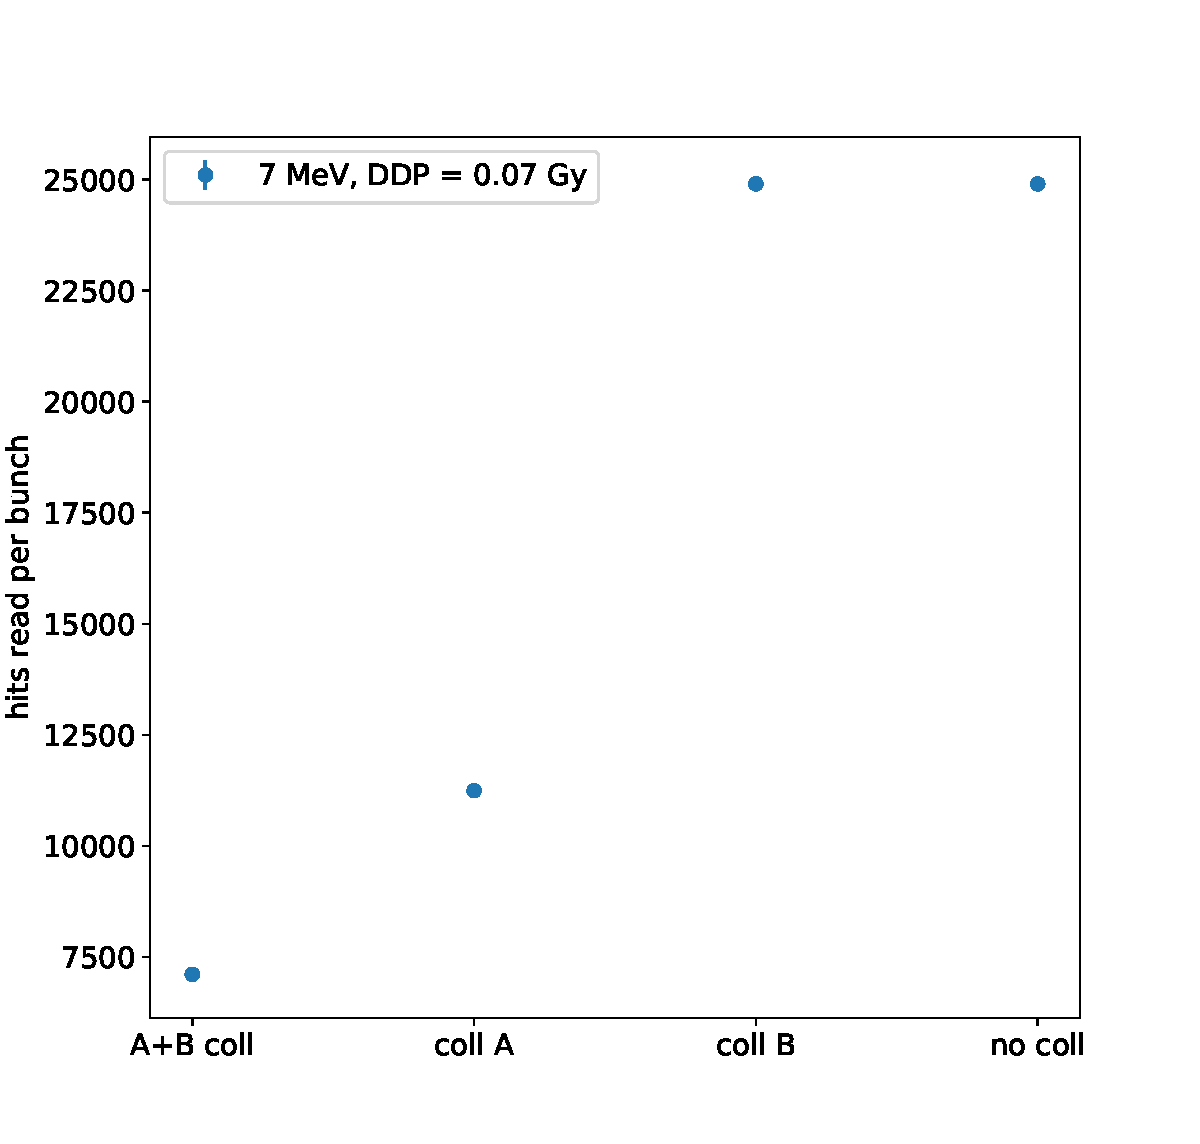
\includegraphics[width=1.1\linewidth]{figures/test_beam/hits.pdf}  
            \column{0.5\textwidth} 
                \begin{itemize}
                    \item Saturation due to the readout system occurs without collimators
                    \item Readout logic has been tested with high hit rate
                \end{itemize}
            \end{columns}
        \end{frame}  